\chapter{Clustering + Association Rules}
\label{chap:experiment3}
\section*{Objective}
Cluster characterization is most difficult part of clustering. Descriptive statistics are the standard way doing it. The objective here is to see if association rules will (hopefully) give a more intuitive explanation.

\section*{Procedure}
\begin{itemize}
\item Create a clustering of the students data set using the marks attributes.
\item KMeans is used and k is determined by using an elbow plot. The elbow plot was reasonably sharp at 4.
\item An extra column is added to the student dataset which contains the id of the cluster to which a particular record belongs to.
\item Association rules are generated by forcing the cluster id to be the antecedent to get the characterization of each cluster.
\end{itemize}

\section*{Observations}
\begin{itemize}
\item Elbow plot obtained

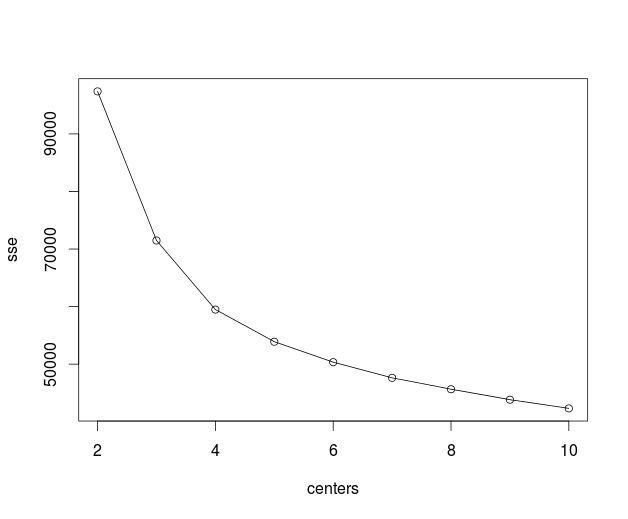
\includegraphics[scale=0.5]{img/kmeans_elbow.png}


\item Distribution around NRC{\_}CLASS
\begin{lstlisting}
       1    2 D    FAIL PASS
  1    1   57    0 2878 8780
  2 4554    0 1439    1    0
  3    0    0    0 4950    5
  4 4386 5669    1   32  249
\end{lstlisting}

\item Characterization using mean marks

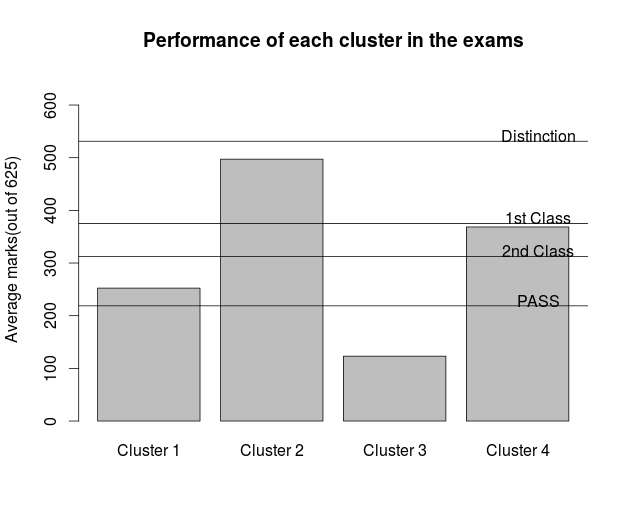
\includegraphics[scale=0.5]{img/barplot_mean_marks.png}


\item Visualization after reducing dimension to two using SVD

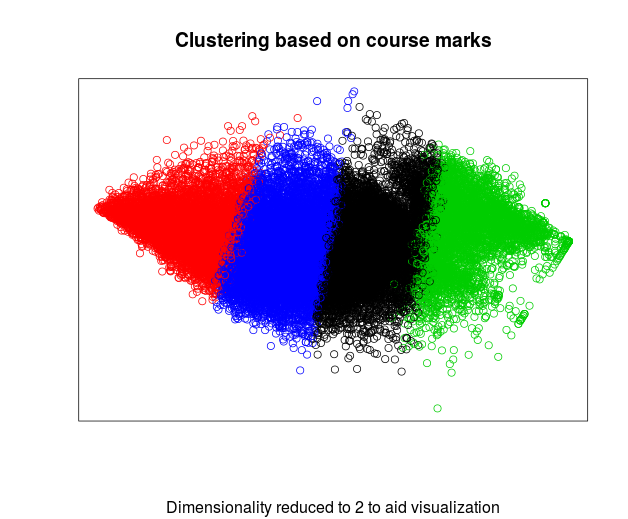
\includegraphics[scale=.5]{img/clusters_marks.png}




\item Association rules for each cluster
\begin{lstlisting}
> inspect(sort(cluster.rules))
   lhs               rhs                          support confidence     lift
1  {CLUSTER_ID=1} => {NRC_PHYSICAL_CONDITION=N} 0.3540695  0.9973540 1.0003245
2  {CLUSTER_ID=1} => {CANDIDATE_TYPE=RF}        0.3011333  0.8482417 0.9576707
3  {CLUSTER_ID=1} => {NRC_MEDIUM=K}             0.2771953  0.7808126 1.1236864
4  {CLUSTER_ID=1} => {NRC_CLASS=PASS}           0.2660445  0.7494025 2.7376336

5  {CLUSTER_ID=2} => {CANDIDATE_TYPE=RF}        0.1815042  0.9993327 1.128253
6  {CLUSTER_ID=2} => {NRC_PHYSICAL_CONDITION=N} 0.1813526  0.9984985 1.001472
7  {CLUSTER_ID=2} => {NRC_CASTE_CODE=4}         0.1536877  0.8461795 1.196368
8  {CLUSTER_ID=2} => {NRC_CLASS=1}              0.1379916  0.7597598 2.804339

9  {CLUSTER_ID=3} => {NRC_CLASS=FAIL}           0.1499909  0.9989909 4.1939573
10 {CLUSTER_ID=3} => {NRC_PHYSICAL_CONDITION=N} 0.1489607  0.9921292 0.9950841
11 {CLUSTER_ID=3} => {S2_CLASS=FAIL}            0.1335374  0.8894046 3.4110554
12 {CLUSTER_ID=3} => {S1_CLASS=FAIL}            0.1203866  0.8018163 3.9028825
13 {CLUSTER_ID=3} => {NRC_MEDIUM=K}             0.1198715  0.7983855 1.1489760
14 {CLUSTER_ID=3} => {L1_CLASS=FAIL}            0.1105994  0.7366297 4.2330232

15 {CLUSTER_ID=4} => {NRC_PHYSICAL_CONDITION=N} 0.3126477  0.9981619 1.001135
16 {CLUSTER_ID=4} => {CANDIDATE_TYPE=RF}        0.3112842  0.9938086 1.122017
17 {CLUSTER_ID=4} => {NRC_CASTE_CODE=4}         0.2308345  0.7369643 1.041954
18 {CLUSTER_ID=4} => {NRC_MEDIUM=K}             0.2207139  0.7046532 1.014084
\end{lstlisting}

\end{itemize}

\section*{Conclusions}
\begin{itemize}
\item Generating association rules on clusters is a satisfactory categorization technique. 
\item The lift is sometimes close to 1 which suggests independence. But this does not matter as the rules are not being interpreted as correlations between the lhs and rhs. The rhs just gives the categorization of the cluster. Lift close to one suggests the same categorization for other clusters.
\item The low support is also not a matter of concern as it is reflective of the measure w.r.t the whole dataset and not to the particular cluster.
\item Categorization : The categorization is as shown in the observations. The physical condition of students across clusters being normal is result of the lopsided distribution.
\end{itemize}
